\chapter{Bruksanvisning}

Stortingets Tibetkomité består av enkeltrepresentanter med et spesielt sterkt 
engasjement for Tibet. Etter stortingsvalget høsten 2013 tok Venstres Ketil 
Kjenseth på seg en koordinerende rolle, og sendte i januar ut en mail til alle 
stortingsrepresentanter om hvem som kunne tenke seg å bidra.
Til tross for at Høyre åpner sitt landsmøte på Gardermoen fredag formiddag har 
fem stortingsrepresentanter fra regjeringspartiet funnet plass i programmet til 
å møte tibetaneren: Michael Tetzschner, Heidi Nordby Lunde, Erik Skutle, Anders 
B. Werp og Peter Chr. Frølich. Også Unge Høyre-leder Paul Joakim Sandøy er med 
og tar imot Dalai Lama.

\section{Kode}
Her kommer litt javakode for å teste ut hvorda det kommer til å se ut.

\begin{lstlisting}[title=Eksempelkode, caption=Koden teller til 1000, label=brakode]
class KnappeLytter implements ActionListener {

        @Override
        public void actionPerformed(ActionEvent e) {
            if (e.getSource().equals(vindu.getLagreButton())) {
                if(erNyregistrering){
                    registrerNyLeietaker();
                }
            } else if (e.getSource().equals(vindu.getAvbrytButton())) {
                vindu.dispose();
            }
        }

    }
\end{lstlisting}


\section{Kode fra fil}
Slik kan man legge inn kode direkte fra en java fil

\lstinputlisting[title=Tellerklasse, caption=Koden her gir NullPointerException, label=java:test1]{./kode/bruksanvisning/1.java}



\section{Liste}
Her kommer eksepel på en liste\footnote{Her legger man til en fotnot hvis man ønsker å kommentere noe.}
\begin{itemize}
 \item Epple
 \item Pære
 \item Frosker
 \item Banan
\end{itemize}



\section{Figurer}
\subsection{Eksempel 2}
\begin{figure}[ht]
 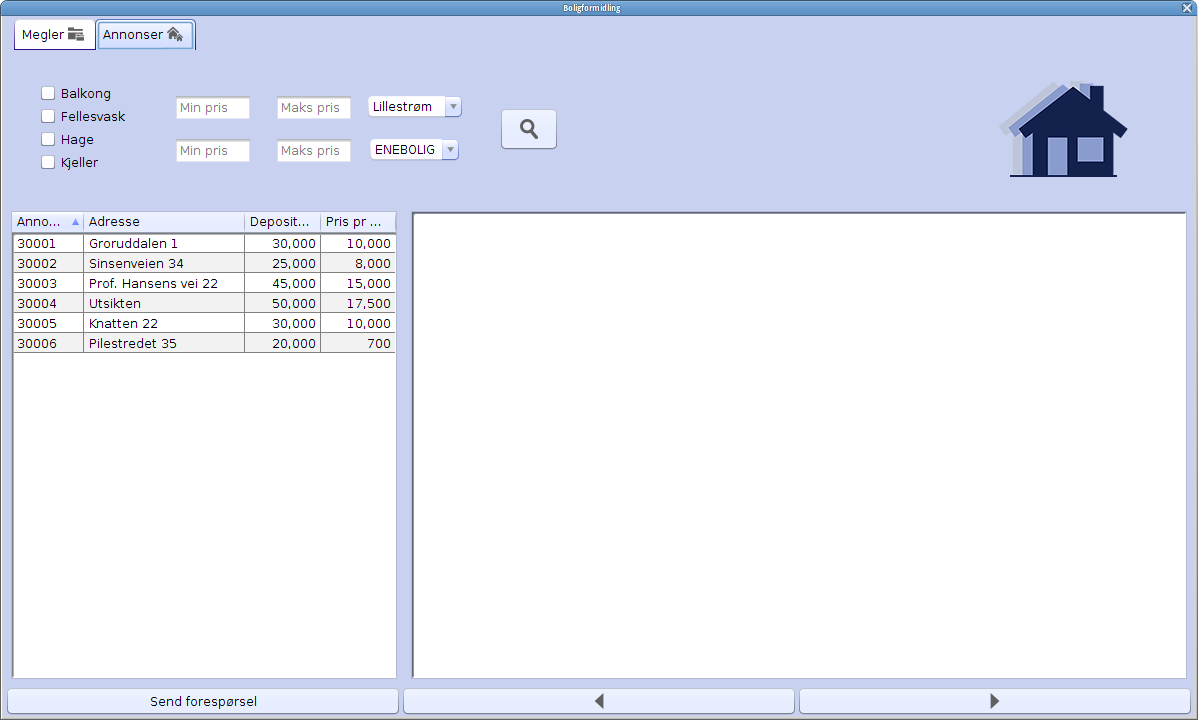
\includegraphics[width=\textwidth,height=\textheight,keepaspectratio]{./img/bruksanvisning/1.png}
 \caption{Dette er et eksempelbilde. Bilde blir automatisk numerert og lagt til i registeret.}
 %Her kommer en kabel for kryssreferering i teksten til figuren
 \label{fig:hovedvindu}
\end{figure}

\section{Referering}
Man må referer til alle figurer og kodeeksempel, som regel skal det ikke finnes en figur eller kodeeksempel dersom man ikke refererer til det i teksten. For at man skal kunne referer til noe så må man ha \textit{label} tag. For eksempel kan man nå referer til bilde gjennom følgende \ref{fig:hovedvindu}. \\
Man kan også ta en referanse til code gjennom \ref{java:test1}

